\documentclass{article}	

\usepackage[utf8]{inputenc}
\usepackage{amsmath}
\usepackage[german]{babel}
\usepackage{amssymb}
\usepackage{amsxtra}
\usepackage[dvips]{epsfig,psfrag}
\usepackage{listings}

\newcommand{\refchapter}[1]{Kapitel~\ref{#1}}
\newcommand{\refsec}[1]{Sektion~\ref{#1}}
\newcommand{\refeqn}[1]{Gleichung~(\ref{#1})}
\newcommand{\reffig}[1]{Abbildung~\ref{#1}}

\title{
{\bf \scriptsize RHEINISCH-WESTF\"ALISCHE TECHNISCHE HOCHSCHULE AACHEN \\
LuFG Informatik 12 (Prof. Dr. rer. nat. Uwe Naumann)}
\vspace{.5cm} \\

\epsfig{file=figures/STCE_Logo_WWW.eps,width=.7\textwidth}
\vspace{1cm} \\
{\bf \Large Korrelation und Regressionsanalyse} \\
{\large Proposal} 
}

\author{vorgelegt von Patrick Neidig (Matr.-Nr. ??????)\\
	und Marius Grysla (Matr.-Nr. 274047)}

\begin{document}

\lstloadlanguages{[ISO]C++}
\lstset{basicstyle=\small, numbers=left, numberstyle=\footnotesize,
  stepnumber=1, numbersep=5pt, breaklines=true, escapeinside={/*@}{@*/}}


\pagestyle{headings}

\maketitle

%\newpage
%\tableofcontents % Brauchen wir für das Proposal ein Inhaltserzeichnis?

\newpage

\section{Einleitung}

\subsection{Motivation}

\section{Korrelation}

\section{Regressionsanalyse}

\subsection{Regressionsmodelle}

\subsection{Analyse}

\section{Zeitplan}

Der Zeitplan für die Seminararbeit und die verschiedenen Präsentationen richtet sich hauptsächlich nach den vorgegebenen Terminen.
Eine Übersicht über die Arbeitsschritte ist in Abbildung \ref{fig:Zeitplan} abgebildet.

\begin{figure}[t]
 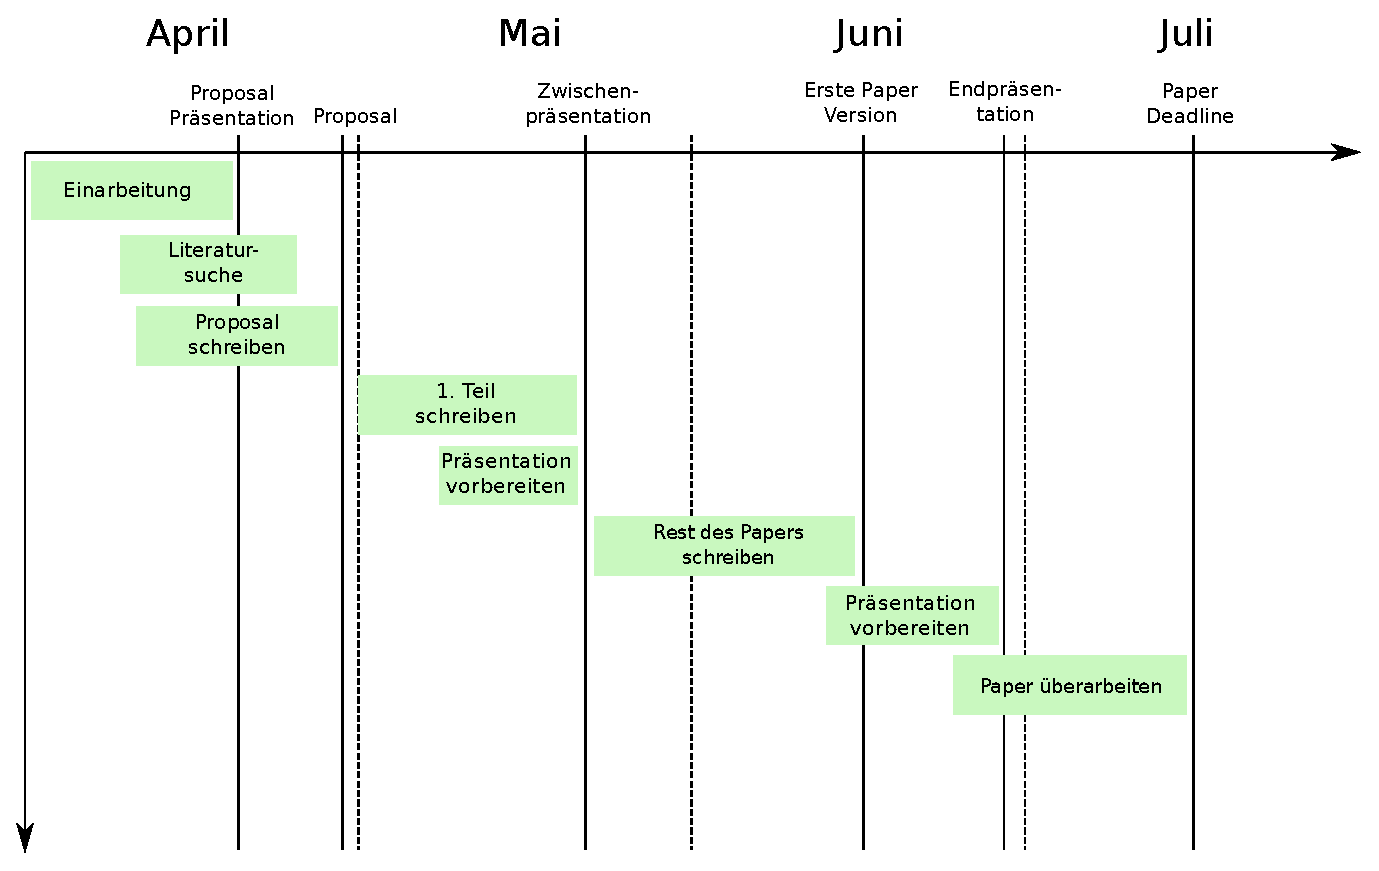
\includegraphics[width=\linewidth]{./figures/Workplan-adj.eps}
 \caption{Der geplante Arbeitsverlauf mit Abgabezeitpunkten.}
 \label{fig:Zeitplan}
\end{figure}



\end{document}

